\documentclass[a4paper, 12pt]{article}
\usepackage[a4paper,top=1.5cm, bottom=1.5cm, left=1cm, right=1cm]{geometry}
\usepackage{cmap}					% поиск в PDF
\usepackage{mathtext} 				% русские буквы в формулах
\usepackage[T2A]{fontenc}			% кодировка
\usepackage[utf8]{inputenc}			% кодировка исходного текста
\usepackage[english,russian]{babel}	% локализация и переносы

\usepackage{amsmath}
\usepackage{indentfirst}
\usepackage{longtable}
\usepackage{graphicx}
\usepackage{array}

\usepackage{wrapfig}
\usepackage{siunitx} % Required for alignment
\usepackage{subfigure}
\usepackage{multirow}
\usepackage{rotating}
\usepackage{caption}

\graphicspath{{.}}


\title{\begin{center}Лабораторная работа №2.1.2\end{center}
Определение $C_p / C_v$ методом адиабатического расширения}
\author{Рожков А. В. \\ Преподаватель Яворский В. А.}
\date{\today}

\begin{document}
    \pagenumbering{gobble}
    \maketitle
    \newpage
    \pagenumbering{arabic}

    \textbf{Цель работы:} определение отношения $C_p / C_v$ углекислого газа по измерения давления в стеклянном сосуде. Измерения производятся сначала после адиабатического расширения газа а затем после нагревания сосуда и газа до комнатной температуры.

	\textbf{В работе используются:} стеклянный сосуд; U-образный водяной манометр $\sigma_h = 0.2~см.вод.ст.$; газгольдер с углекислым газом; секундомер $\sigma_t = 0.3~с$.

	\begin{figure}[b!]	\label{plan2}

		\center{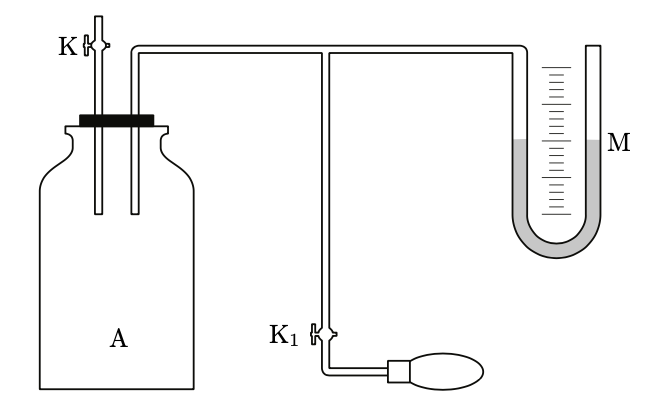
\includegraphics[width=1 \linewidth]{img/ust.jpg}}
		\caption{Установка для определения $C_p / C_v$ методом адиабатического расширения газа}

	\end{figure}

	\section{Экспериментальная установка}

		Используемая для опытов экспериментальная установка состоит из стеклянного сосуда А (объёмом около 20 л), снабженного краном К, и U-образного жидкостного манометра, измеряющего избыточное давление газа в сосуде. Схема установки показана на Рис. 1.

		Избыточное давление создаётся с помощью резиновой груши, соединённой с сосудом трубкой с краном $К_1$.

		В начале опыта  в стеклянном сосуде А находится исследуемый газ при комнатной температуре $T_1$ и давлении $P_1$, несколько превышающем атмосферное давление  $P_0$. После открытия крана К, соединяющего сосуд А с атмосферой, давление и температура газа будут понижаться. Это уменьшение температуры приближённо можно считать адиабатическим.

		Для адиабатического процесса можно записать следующее уравнение:

		\begin{equation}\label{mk}
		\left(\dfrac{P_1}{P_2}\right)^{\gamma - 1} = \left(\dfrac{T_1}{T_2}\right)^\gamma ,
		\end{equation}

		где индексом "1" обозначено состояние после повышения давления в сосуде и выравнивания температуры с комнатной, а индексом "2"  $-$ сразу после открытия крана и выравнивания давления с атмосферным.

		После того, как кран К вновь отсоединит сосуд от атмосферы , происходит медленное изохорическое нагревание газа со скоростью, определяемой теплопроводностью стеклянных стенок сосуда. Вместе с ростом температуры растёт и давление газа. З время порядка $\Delta t_T$  (время установления температуры) система достигает равновесия, и установившаяся температура газа $T_3$ становится равной комнатной температуре $T_1$.

		Тогда используя закон Гей-Люссака для изохорического процесса и уравнение \eqref{mk} найдём $\gamma$:

		\begin{equation}\label{acc}
		\gamma = \dfrac{\ln(P_1 / P_0)}{\ln (P_1 / P_3)}.
		\end{equation}

		С учётом того, что $P_i = P_0 + \rho g h_i$ и пренебрегая членами второго порядка малости получим из \eqref{acc}:

		\begin{equation}\label{r}
		\gamma \approx \dfrac{h_1}{h_1 - h_2}.
		\end{equation}

	\section{Ход работы}

		\subsection{Проверка герметичности установки и определение времени установления равновесия}

			Открываем кран между баллоном и газгольдером с углекислым газом. Увеличение давления в сосуде сопровождается повышением температуры. По манометру давление составляет $10.7~мм.вод.ст.$. После закрытия крана давление начинает падать в связи с охлаждением углекислого газа от стенок сосуда. Зависимость давления от времени представлено на графике \ref{plot:h_t_1} и в таблице \ref{table:h_t_1}.

			\begin{figure}[ht!]
				\begin{minipage}[c]{.6\linewidth}
					\centering
					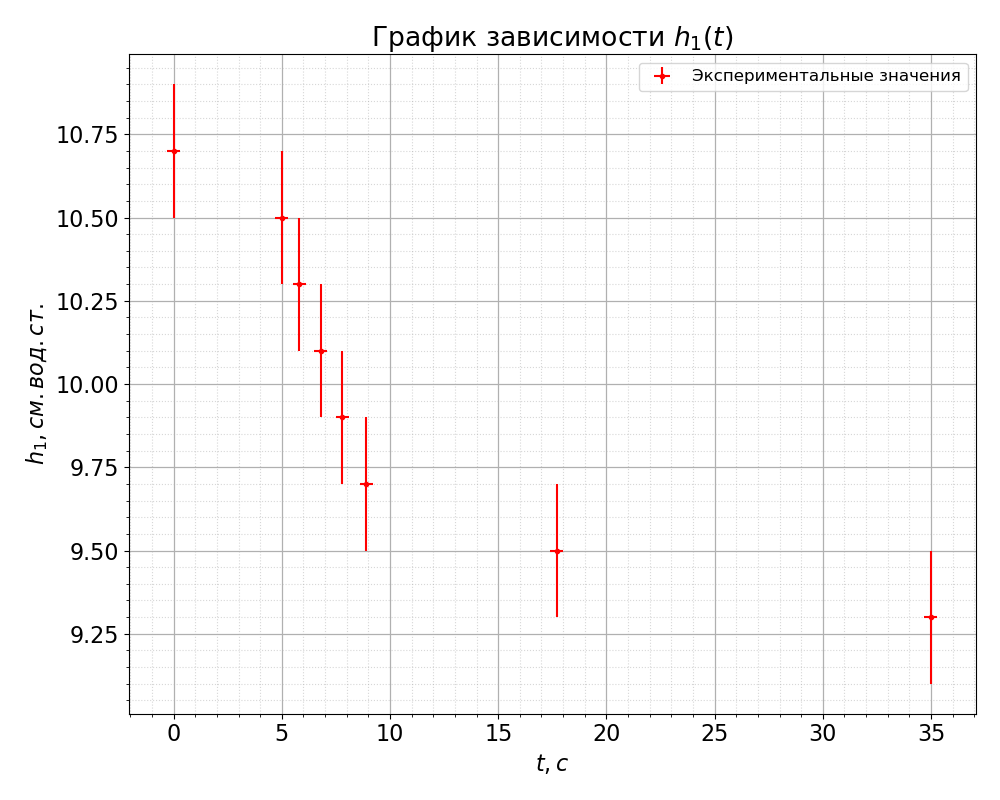
\includegraphics[width=1.0\linewidth]{img/plot_h1_t_1.png}
					\captionof{figure}{График зависимости давления от времени}
					\label{plot:h_t_1}
				\end{minipage}\hfill
				\begin{minipage}[c]{.3\linewidth}
					\centering
					\begin{tabular}{|c|c|}
						\hline

						$t, с$ & $h_1, см.вод.ст.$\\ \hline
						0.0 & 10.7\\ \hline
						5.0 & 10.5\\ \hline
						5.8 & 10.3\\ \hline
						6.8 & 10.1\\ \hline
						7.8 & 9.9\\ \hline
						8.9 & 9.7\\ \hline
						17.7 & 9.5\\ \hline
						35.0 & 9.3\\ \hline

					\end{tabular}
					\captionof{table}{Зависимость давления от времени}
					\label{table:h_t_1}
				\end{minipage}
			\end{figure}

			Давление установилось через 35 секунд. Наблюдали ещё 55 секунд, показания не менялись. Для следующих измерений возьмём время установления равновесия $\Delta t_T \sim 70~с$.

		\subsection{Измерение показателя адиабаты для разных времён открытия крана}

			После наполнения баллона ждём время $\Delta t_T$. Фиксируем давление $h_1$ и открываем кран с атмосферой на $\Delta t_p \sim 0.5~с$ (это время достигается быстрым поворотом крана на $180^o$). Затем снова ждём время $\Delta t_T$ и фиксируем $h_2$. Проведём серию из 10 измерений. Результаты в таблице \ref{table:gamma_1}.

			Приборная погрешность показателя адиабаты по формуле:
			$$
				\sigma_{\gamma}^{приб} = \sigma_h \frac{\gamma}{h_1 - h_2} \sqrt{\left( \frac{h_2}{h_1} \right)^2 + 1}
			$$

			\begin{table}[!ht]
				\centering
				\begin{tabular}{|c|c|c|}
					\hline

					$h_1, см.вод.ст.$ & $h_2, см.вод.ст.$ & $\gamma$\\ \hline
					9.3 & 2.0 & $(1.27 \pm 0.04)$\\ \hline
					9.3 & 2.0 & $(1.27 \pm 0.04)$\\ \hline
					9.5 & 2.2 & $(1.30 \pm 0.04)$\\ \hline
					9.5 & 2.2 & $(1.30 \pm 0.04)$\\ \hline
					9.3 & 2.0 & $(1.27 \pm 0.04)$\\ \hline
					9.5 & 2.2 & $(1.30 \pm 0.04)$\\ \hline
					9.5 & 2.4 & $(1.34 \pm 0.04)$\\ \hline
					9.5 & 2.2 & $(1.30 \pm 0.04)$\\ \hline
					9.3 & 2.2 & $(1.31 \pm 0.04)$\\ \hline
					9.5 & 2.4 & $(1.34 \pm 0.04)$\\ \hline
					\multicolumn{2}{|r|}{\textbf{Среднее:}} & $\boldsymbol{(1.30 \pm 0.04)}$ \\ \hline

				\end{tabular}
				\caption{Показатель адиабаты для $\Delta t_p \sim 0.5~с$}
				\label{table:gamma_1}
			\end{table}

			Далее аналогично проведём по 2 измерения для различных времён открытия крана.

			\begin{figure}[ht!]
				\begin{minipage}[c]{.49\linewidth}
					\centering
					\begin{tabular}{|c|c|c|}
						\hline

						$h_1, см.вод.ст.$ & $h_2, см.вод.ст.$ & $\gamma$\\ \hline
						9.5 & 2.2 & $(1.30 \pm 0.04)$\\ \hline
						9.5 & 2.4 & $(1.34 \pm 0.04)$\\ \hline
						\multicolumn{2}{|r|}{\textbf{Среднее:}} & $\boldsymbol{(1.32 \pm 0.04)}$ \\ \hline

					\end{tabular}
					\captionof{table}{Показатель адиабаты для $\Delta t_p \sim 2~с$}
					\label{table:gamma_2}

				\end{minipage} \hfill
				\begin{minipage}[c]{.49\linewidth}
					\centering
					\begin{tabular}{|c|c|c|}
						\hline

						$h_1, см.вод.ст.$ & $h_2, см.вод.ст.$ & $\gamma$\\ \hline
						9.5 & 2.2 & $(1.30 \pm 0.04)$\\ \hline
						9.3 & 2.0 & $(1.27 \pm 0.04)$\\ \hline
						\multicolumn{2}{|r|}{\textbf{Среднее:}} & $\boldsymbol{(1.29 \pm 0.04)}$ \\ \hline

					\end{tabular}
					\captionof{table}{Показатель адиабаты для $\Delta t_p \sim 4~с$}
					\label{table:gamma_3}
				\end{minipage}
			\end{figure}

			\begin{figure}[ht!]
				\begin{minipage}[c]{.49\linewidth}
					\centering
					\begin{tabular}{|c|c|c|}
						\hline

						$h_1, см.вод.ст.$ & $h_2, см.вод.ст.$ & $\gamma$\\ \hline
						9.1 & 1.8 & $(1.25 \pm 0.03)$\\ \hline
						9.5 & 2.0 & $(1.27 \pm 0.03)$\\ \hline
						\multicolumn{2}{|r|}{\textbf{Среднее:}} & $\boldsymbol{(1.26 \pm 0.04)}$ \\ \hline

					\end{tabular}
					\captionof{table}{Показатель адиабаты для $\Delta t_p \sim 6~с$}
					\label{table:gamma_4}

				\end{minipage} \hfill
				\begin{minipage}[c]{.49\linewidth}
					\centering
					\begin{tabular}{|c|c|c|}
						\hline

						$h_1, см.вод.ст.$ & $h_2, см.вод.ст.$ & $\gamma$\\ \hline
						9.5 & 1.8 & $(1.23 \pm 0.03)$\\ \hline
						9.1 & 1.8 & $(1.25 \pm 0.03)$\\ \hline
						\multicolumn{2}{|r|}{\textbf{Среднее:}} & $\boldsymbol{(1.24 \pm 0.03)}$ \\ \hline

					\end{tabular}
					\captionof{table}{Показатель адиабаты для $\Delta t_p \sim 8~с$}
					\label{table:gamma_5}
				\end{minipage}
			\end{figure}

			\begin{table}[!ht]
				\centering
				\begin{tabular}{|c|c|c|}
					\hline

					$h_1, см.вод.ст.$ & $h_2, см.вод.ст.$ & $\gamma$\\ \hline
					9.3 & 1.8 & $(1.24 \pm 0.03)$\\ \hline
					9.3 & 1.6 & $(1.21 \pm 0.03)$\\ \hline
					\multicolumn{2}{|r|}{\textbf{Среднее:}} & $\boldsymbol{(1.22 \pm 0.04)}$ \\ \hline

				\end{tabular}
				\captionof{table}{Показатель адиабаты для $\Delta t_p \sim 10~с$}
				\label{table:gamma_6}
			\end{table}

		\subsection{Получение окончательного результата экстраполяцией зависимости $\gamma$ от $\Delta t_p$ к значению $\Delta t_p = 0$}

		Построим график $\gamma(\Delta t_p)$ и по нему при помощи МНК определим значение $\gamma$ углекислого газа.

		\begin{figure}[!ht]
			\begin{center}
				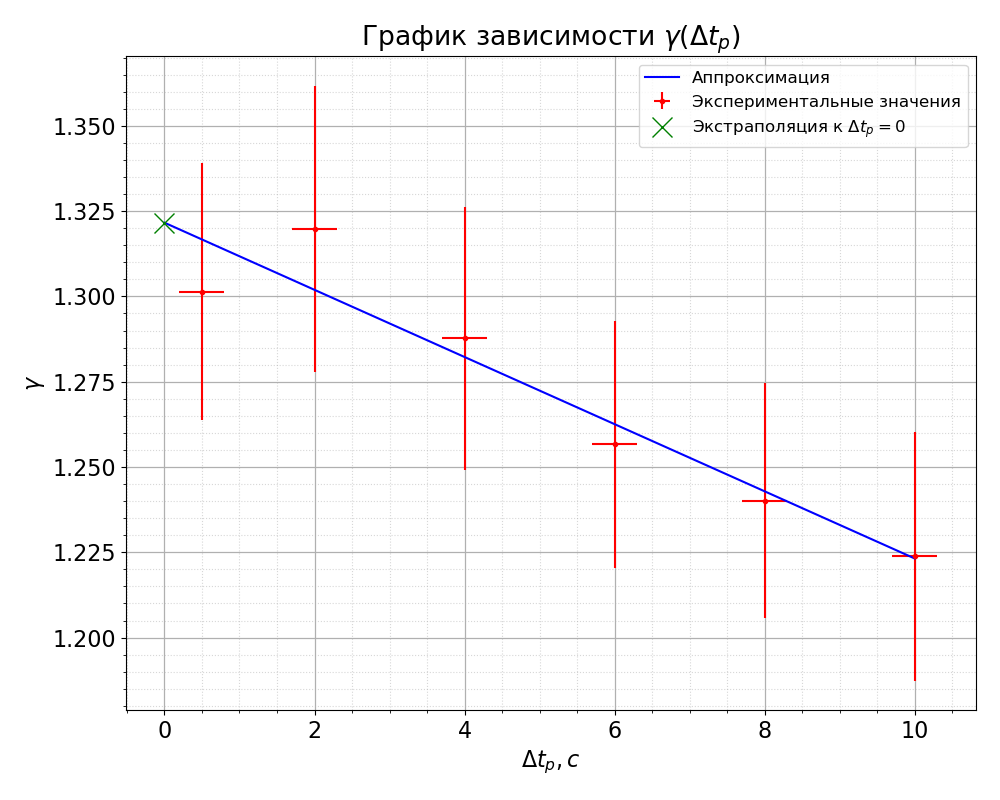
\includegraphics[width=0.6 \textwidth]{img/plot_gamma_t.png}
			\end{center}
			\caption{График зависимости $\gamma$ от $\Delta t_p$}
			\label{plot:gamma_t}
		\end{figure}

		Полная погрешность результата по формуле:
		$$
			\sigma_{\gamma_{итог}} = \sqrt{\sigma_{\gamma}^2 + \left( \Delta t_p \sigma_k \right)^2 + \left( k \sigma_{\Delta t_p} \right)^2 + \sigma_k^{случ^2}}
		$$

		Итого:
		$$
			\gamma_{итог} = (1.32 \pm 0.04)
		$$

		Табличное значение показателя адиабаты для углекислого газа составляет $1.30$.

	\section{Вывод}

		Определили отношение $C_p / C_v$ углекислого газа по измерению давления в стеклянном сосуде.

		Результат совпал с табличным значением в пределах погрешности. Значит метод экстраполяции зависимости к нулевому времени истечения газа оправдан, так как полученное значение при наибольшем времени открытия крана ($10~с$) составило $1.22 \pm 0.04$, что существенно отличается от табличного значения.

\end{document}
